\documentclass[aspectratio=169,12pt]{beamer}

\usetheme{Madrid}
\usecolortheme{seahorse}
\setbeamertemplate{navigation symbols}{}
\setbeamertemplate{footline}[frame number]

\usepackage{amsmath,amssymb}
\usepackage{graphicx}
\usepackage{xcolor}
\usepackage{tikz}
\usetikzlibrary{arrows.meta,positioning}
\usepackage{listings}

\graphicspath{{../../plots/}}

\definecolor{topological}{HTML}{1f77b4}
\definecolor{critical}{HTML}{2ca02c}
\definecolor{trivial}{HTML}{d62728}
\definecolor{edgemode}{HTML}{e377c2}
\definecolor{codebg}{HTML}{f5f5f5}
\definecolor{codekw}{HTML}{0000cd}
\definecolor{codecomment}{HTML}{228b22}
\definecolor{codestring}{HTML}{8b0000}

\lstset{
  language=Python,
  basicstyle=\ttfamily\scriptsize,
  keywordstyle=\color{codekw}\bfseries,
  commentstyle=\color{codecomment}\itshape,
  stringstyle=\color{codestring},
  backgroundcolor=\color{codebg},
  frame=single,
  showstringspaces=false,
  breaklines=true
}

\newcommand{\ket}[1]{|#1\rangle}
\newcommand{\Oedge}{X_0Z_1\cdots Z_{L-2}X_{L-1}}
\newcommand{\E}{\mathcal{E}}

\title[Kitaev Chain -- Block 4]{Majorana Modes in the Machine}
\subtitle{Week 8: NISQ Reality Check -- Noise Model and Failure Modes}
\author{Dobromir Stoev\\ Edgar Harutyunyan\\ Guilherme Schewtschik\\ Jaskaran Singh\\ Zhengyi Liu\\ Zhenming Shi}
\institute{Advanced Seminar -- AI-Augmented Theoretical Physics}
\date{\today}

\begin{document}

\begin{frame}
 \titlepage
\end{frame}

\begin{frame}{What Week 7 Gives Us}
  \begin{columns}[T]
    \begin{column}{0.62\textwidth}
      \centering
      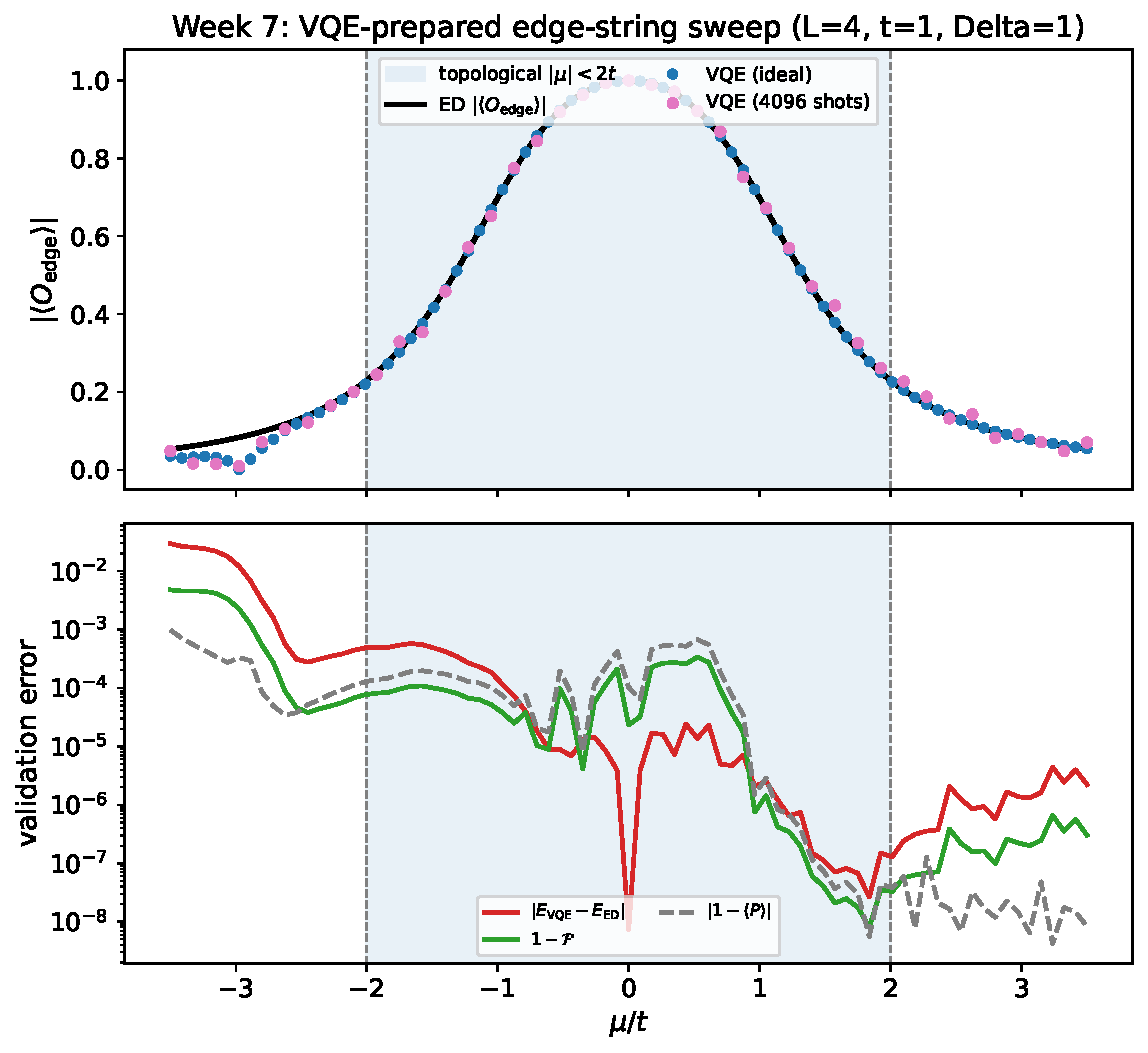
\includegraphics[width=\textwidth,height=0.82\textheight,keepaspectratio]{block3_week7_vqe_sweep.pdf}
    \end{column}
    \begin{column}{0.34\textwidth}
      \small
      \textbf{Noiseless baseline}
      \begin{itemize}
        \item Prepared by parity-constrained VQE
        \item Edge string measured ideally and with shots
        \item ED validates energy, parity, fidelity, string value
      \end{itemize}
    
    \end{column}
  \end{columns}
\end{frame}

\begin{frame}{What Noise Can Break}
  \begin{columns}[T]
    \begin{column}{0.48\textwidth}
      \textbf{State preparation}
      \begin{itemize}
        \item VQE ansatz gates no longer implement exactly $U(\theta)$.
        \item Entangling-gate errors reduce edge coherence.
        \item Relaxation can bias the parity sector.
      \end{itemize}
    \end{column}
    \begin{column}{0.48\textwidth}
      \textbf{Measurement}
      \begin{itemize}
        \item Readout flips corrupt the bitstring parity product.
        \item Shot noise broadens the string estimator.
        \item A small true signal becomes hard to distinguish from zero.
      \end{itemize}
    \end{column}
  \end{columns}

  \begin{alertblock}{Main risk}
    Noise can flatten the edge-string contrast between $|\mu|<2t$ and $|\mu|>2t$, even when the noiseless circuit is correct.
  \end{alertblock}
\end{frame}

\begin{frame}{Noise Channels to Add}
  \begin{center}
  \begin{tabular}{p{0.25\textwidth}p{0.33\textwidth}p{0.32\textwidth}}
    \textbf{Channel} & \textbf{Physical meaning} & \textbf{Expected effect} \\
    \hline
    Depolarizing error & Random Pauli error after gates & Shrinks correlations and string contrast \\
    Readout error & Classical bit flip during measurement & Biases $\pm1$ parity-product estimator \\
    Amplitude damping & $T_1$ relaxation toward $\ket{0}$ & Can change particle number and parity balance \\
    Phase damping & $T_2$ dephasing & Destroys coherent edge-to-edge correlations
  \end{tabular}
  \end{center}

\end{frame}

\begin{frame}{Two Experiments to Keep Separate}
  \begin{columns}[T]
    \begin{column}{0.48\textwidth}
      \textbf{Frozen-parameter noise test}
      \begin{itemize}
        \item Use $\theta^*(\mu)$ from noiseless Week 7.
        \item Add noise only during circuit execution.
        \item Measures readout and circuit degradation at fixed preparation.
      \end{itemize}
    \end{column}
    \begin{column}{0.48\textwidth}
      \textbf{Noisy optimization test}
      \begin{itemize}
        \item Optimize the VQE cost under noisy estimates.
        \item Tests whether the optimizer can still find good parameters.
        \item Harder and more expensive; should come second.
      \end{itemize}
    \end{column}
  \end{columns}

  \begin{block}{Engineering rule}
    First isolate measurement/circuit degradation; only then study optimizer degradation.
  \end{block}
\end{frame}

\begin{frame}{Circuit-Level Noise Protocol: Formalism}
    \textbf{Objective:} Formalize the mapping from the noiseless VQE sweep to the noisy density matrix.
    
    \vspace{0.3cm}
    For the Week 7 optimized parameters $\theta^*(\mu)$, the ideal pure state is $\rho_{\text{id}} = \dyad{\psi(\theta^*)}$. We define the physical execution via completely positive trace-preserving (CPTP) maps:
    
    \begin{equation}
        \rho_{\text{noisy}} = \mathcal{E}_{\text{readout}} \circ \mathcal{E}_{\text{meas-basis}} \circ \mathcal{E}_{\text{gate}} (\rho_{\text{id}})
    \end{equation}
    
    \begin{itemize}
        \item \textbf{Gate Noise ($\mathcal{E}_{\text{gate}}$):} Modeled via local depolarizing channels after each 2-qubit gate. $\mathcal{D}_p(\rho) = (1-p)\rho + \frac{p}{4^2-1}\sum_{i \neq 0} P_i \rho P_i$.
        \item \textbf{Basis Rotation ($\mathcal{E}_{\text{meas-basis}}$):} Ideal unitary mapping for $X_0Z_1Z_2X_3$.
        \item \textbf{Readout Assignment ($\mathcal{E}_{\text{readout}}$):} Asymmetric bit-flip channel $p(0|1)$ and $p(1|0)$ applied to the diagonal elements of the density matrix.
    \end{itemize}
\end{frame}

\begin{frame}{Frozen-Parameter Test: Readout vs. Depolarizing Channels}
    \textbf{Protocol:} Evaluate $\text{Tr}(\hat{O}_{\text{edge}} \rho_{\text{noisy}})$ using frozen $\theta^*(\mu)$ from the ED/ideal VQE baseline.
    
    \vspace{0.2cm}
    \begin{columns}
        \begin{column}{0.45\textwidth}
            \textbf{Expected Behavior:}
            \begin{itemize}
                \item The ideal ED baseline peaks at $\langle O_{\text{edge}} \rangle = 1.0$ at $\mu=0$.
                \item \textit{Readout error alone} linearly scales the entire curve by $(1-2\epsilon)^4$, preserving the functional shape.
                \item \textit{Gate noise} broadens the variance $\text{Tr}(\rho^2) < 1$, flattening the topological contrast disproportionately near the critical point $\mu_c = \pm 2t$.
            \end{itemize}
        \end{column}
        \begin{column}{0.5\textwidth}
            % Placeholder for the actual hardware/simulator plot
            \begin{center}
            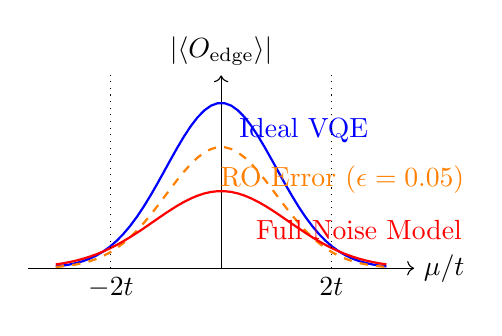
\begin{tikzpicture}[scale=0.7]
                % Axes
                \draw[->] (-3.5,0) -- (3.5,0) node[right] {$\mu/t$};
                \draw[->] (0,0) -- (0,3.5) node[above] {$|\langle O_{\text{edge}} \rangle|$};
                
                % Ideal Curve (Gaussian-like)
                \draw[thick, blue] plot[domain=-3:3, samples=50] (\x, {3*exp(-\x*\x/2)});
                \node[blue] at (1.5, 2.5) {Ideal VQE};
                
                % Noisy Curve 1 (Readout only)
                \draw[thick, orange, dashed] plot[domain=-3:3, samples=50] (\x, {2.2*exp(-\x*\x/2)});
                \node[orange] at (2.2, 1.6) {RO Error ($\epsilon=0.05$)};

                % Noisy Curve 2 (Gate + Readout)
                \draw[thick, red] plot[domain=-3:3, samples=50] (\x, {1.4*exp(-\x*\x/3)});
                \node[red] at (2.5, 0.7) {Full Noise Model};
                
                % Critical points
                \draw[dotted] (-2,0) -- (-2,3.5);
                \draw[dotted] (2,0) -- (2,3.5);
                \node[below] at (-2,0) {$-2t$};
                \node[below] at (2,0) {$2t$};
            \end{tikzpicture}
            \end{center}
        \end{column}
    \end{columns}
\end{frame}

\begin{frame}{Phase-Boundary Failure Criterion}
    We must define mathematically when the topological transition at $|\mu| = 2t$ becomes indistinguishable from the trivial vacuum due to the combined noise channels.
    
    \vspace{0.4cm}
    \textbf{Failure Criterion:} The diagnostic is considered to have failed when the topological signal inside the bulk ($|\mu| < 2t$) cannot be resolved from the statistical and hardware noise floor with a $3\sigma$ confidence interval.
    
    \vspace{0.2cm}
    Specifically, failure occurs if the maximum observable contrast satisfies:
    \begin{equation}
        \max_{\mu} \left| \langle \hat{O}_{\text{edge}}(\mu) \rangle_{\text{meas}} \right| \leq \frac{3}{\sqrt{N_{\text{shots}}}} + \delta_{\text{SPAM}}
    \end{equation}
    where $\delta_{\text{SPAM}}$ is the systematic bias inferred from the parity drift observable, $|1 - \langle \hat{P} \rangle_{\text{noisy}}|$. 
    
\end{frame}
\begin{frame}{Next Week}
  \begin{alertblock}{Next milestone}
    After the frozen-parameter tests, run noisy VQE optimization and compare raw versus mitigated readout.
  \end{alertblock}
\end{frame}

\end{document}
